\chapter{Matheuristics}

A heuristic, as defined in \cite{wiki:Heuristic}, is "any approach to problem-solving or self-discovery that employs a practical method, not guaranteed to be optimal, perfect, logical, or rational, but sufficient for reaching an immediate goal. When finding an optimal solution is impossible or impractical, heuristic methods can speed up the process of finding a satisfactory solution." According to this definition, heuristic algorithms aim to find good solutions in a reasonable time by sacrificing optimality.

Matheuristic algorithms combine heuristic methods with mathematical programming, introducing new constraints to the model. In this way the B\&C algorithm is treated as a black box, making the method independent from its implementation and from the problem. The most representative algorithm of this method is Soft Fixing (see Section \ref{chap:local_branching}).

During the solution computation, CPLEX employs various heuristic and matheuristic algorithms. By adjusting certain parameters, it is possible to change the frequency of their application or the time allocated to them.


\section{Hard Fixing}
The Hard Fixing Heuristic is an iterative approach that fixes certain variables (edges) of a reference solution computed by CPLEX and then attempts to solve the resulting simplified problem using a Mixed-Integer Programming (MIP) solver. The heuristic consists of the following steps:

\begin{enumerate}
    \item Start from a solution
    \item Fix used edges to 1 with a certain probability
    \item Run MIP solver as a black box
    \item Compare solutions and keep the best one
    \item Remove fixed edges
    \item Repeat from point 2
\end{enumerate}

These steps are repeated for a fixed number of iterations. Upon finding a solution, the fixed edges are unfixed, and the process is restarted until the time limit is reached. The optimization is accelerated because the fixed edges removes a lot of feasible solutions from the domain (the nodes of a fixed edges have one degree of freedom less than before). However, optimality of the solution is not guaranteed. Importantly, each iteration's solution is at least as good as or better than the previous one.

The heuristic begins by creating the model and calling the MIP start function that generates a solution using Nearest Neighbor and the 2-opt. This initial solution is likely far from optimal, but we use it to choose some random edges and fix them to 1 by adding a costraint \(x_e=1 \) to the model with a certain probability.

The percentage of edges to be fixed varies at each iteration. Generally, a high percentage is used in the initial iterations and is gradually reduced in subsequent ones, allowing CPLEX greater flexibility in computing the solution. The random selection of edges in Phase 2 ensures the algorithm terminates, as the same variables are not always fixed.

In the implemented version, the percentages used are calculated on the fly, based on how much the results improve at each iteration (a low improvement makes the percentage of free edges increase by 10\%, up to 50\%, allowing the solver to have a higher flexibility).

An example of the solution space exploration using this technique is shown in Figure \ref{fig:hrd_fix}. The pseudo-code of the Hard Fixing Heuristic is provided in Algorithm \ref{alg:hard_fixing}.

\begin{figure}[H]
    \centering
    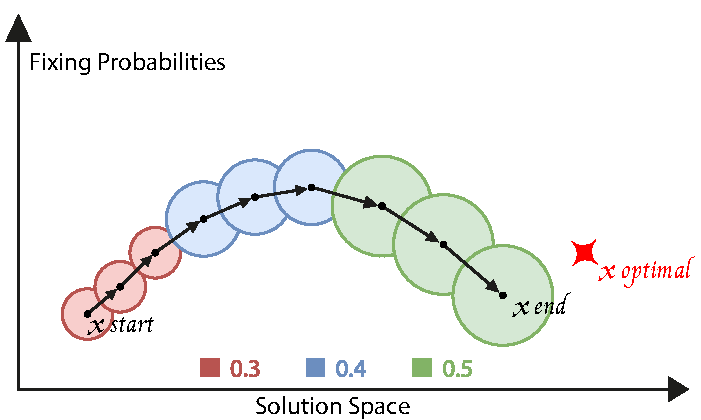
\includegraphics[width=0.8\linewidth]{Immagini/hrd_fix.pdf}
    \caption{Solution space exploration using the Hard Fixing Heuristic.}
    \label{fig:hrd_fix}
\end{figure}

\begin{algorithm}[H]
    \caption{Hard Fixing}
    \label{alg:hard_fixing}
    \begin{spacing}{1.2} % Adjust this value to change line spacing
        \KwIn{TSP Instance}
        \KwOut{A valid tour}
        \BlankLine
        build cplex model\;
        current\_solution $\leftarrow$ addMipStart\;
        freeEdgesProb $\leftarrow$ 0.1\;
        \BlankLine
        \While{current time $<$ inst.time\_limit}
        {
            \ForEach{edge of current\_solution}
            {
                \If{edge $=$ 1}
                {
                    fix edge to 1 with probability 1 - freeEdgesProb\;
                }
            }
            \BlankLine\BlankLine
            \textit{cpx\_solution} $\leftarrow$ \textbf{call} branch\&Bound black box\;
            \BlankLine\BlankLine
            \If{cpx\_solution cost \leq \ current\_solution cost}
            {
                \textit{current\_solution} $\leftarrow$ \textit{cpx\_solution}\;
                addMipStart(\textit{current\_solution})\;
            }
            \BlankLine
            \For{each edge of current\_solution}
            {
                free edge\;
            }
            \BlankLine
            \If{$|$objval - cpx\_objval$| < 0.1 \times$ objval}
            {
                freeEdgesProb $\leftarrow$ min(freeEdgesProb + 0.1, 0.5)\;
            }
        }
    \end{spacing}
\end{algorithm}

\section{Local Branching}
\label{chap:local_branching}

The Local Branching method, also known as Soft Fixing, introduced by M. Fischetti \cite{Fischetti2003}, adopts an approach similar to Hard Fixing. However, in this technique, the selection of variables to be set to 1 is not done randomly but is determined by CPLEX.

\newpage

\noindent Starting from a feasible integer solution for the TSP, denoted as \(xH\), which is represented as a binary vector (e.g., [0, 1, 0, ...]) of length \(|E|\), a constraint is applied to the variables with value 1:

\begin{equation}
    \sum_{e \in E\ :\ x_{e}^{H}} x_e \geq n - k
    \label{eq:loc_fix_2}
\end{equation}

where the summation represents the count of variables that are set to 1 in \(xH\) and will remain unchanged, \(n\) denotes the number of edges selected in \(xH\) and where \(k = 2, \ldots, 20\) signifies the degrees of freedom for CPLEX in finding the new solution. In each iteration of the algorithm, a new Local Branching constraint is introduced based on the current solution provided by CPLEX, while the constraint from the previous iteration is removed.

Unlike Hard Fixing, where branches are selected randomly, if there is no improvement in cost and thus no change in the solution, the branches chosen by CPLEX with the new constraint would be the same as in the previous iteration. To overcome this, the value of \(k\) starts at 2 and is incremented if the solution does not improve.
Experimental results indicate that this method helps CPLEX converge more rapidly to the optimal solution, and values of \(k\) greater than 20 do not yield better outcomes. Typically, to explore the solution space, it is necessary to enumerate all the elements within it. The addition of a Local Branching constraint simplifies and accelerates this operation.
Given a feasible integer solution \(xH\) and using the Hamming distance, the \(k\)-opt solutions relative to \(xH\) are those at a distance \(k\) from it as shown in Figure \ref{fig:soft_fix}.

\begin{figure}[H]
    \centering
    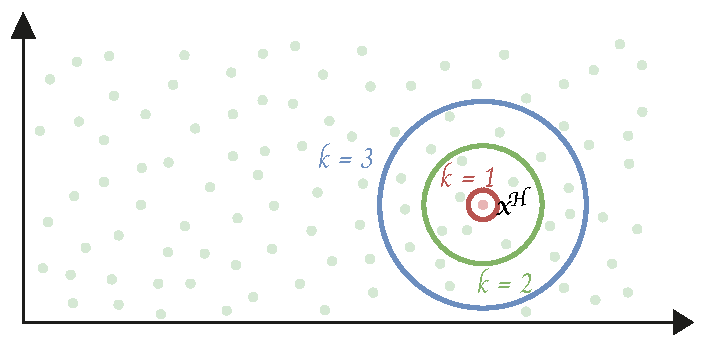
\includegraphics[width=0.8\linewidth]{Immagini/soft_fix.pdf}
    \caption{Solution space and Hamming distance.}
    \label{fig:soft_fix}
\end{figure}

For generic \(k\), approximately \(n^k\) solutions should be generated at a distance \(k\) from \(xH\). These solutions must be analyzed to find one with a lower cost than \(xH\).
Local Branching can also be applied to general problems, not just the TSP. Given an approximate (heuristic) solution \(xH\) for an optimization problem, the mathematical formulation that generates solutions at a distance less than or equal to \(R\) through Local Branching is:

\begin{align}[H]
    min\{c^Tx\ : \ Ax=b,\ x \in \{0,1\}^n\} \label{eq:loc_fix_2} \\[2em]
    H(x,x^h)\ = \sum_{j \in E\ :\ x_{j}^{H}=0} x_j\ + \sum_{j \in E\ :\ x_{j}^{H}=1} 1 - x_j\ \ \leq R \label{eq:loc_fix_2}
\end{align}

Equation \ref{eq:loc_fix_2} represents the Hamming distance of the new solution \(x\) from \(xH\). The goal of Soft Fixing is to improve the solution cost by examining the nearest solutions in the space. The algorithm resembles the hard-fix approach, but instead of using the fixing-probability, we modify the neighborhood by adjusting the radius parameter \(k\). The pseudo-code for Soft Fixing is presented in Algorithm \ref{alg:soft_fixing_algo}.\\

\begin{algorithm}[H]
    \caption{Local Branching}
    \label{alg:soft_fixing_algo}
    \begin{spacing}{1.2} % Adjust this value to change line spacing
        \KwIn{TSP Instance}
        \KwOut{An improved solution}
        \BlankLine
        build cplex model\;
        current\_solution $\leftarrow$ addMipstart\;
        $k \leftarrow 20$\;
        \BlankLine
        \While{current time $<$ inst.time\_limit}
        {
            Add constraint to fix $n-k$ edges\;
            \BlankLine
            \textit{cpx\_solution} $\leftarrow$ \textbf{call} Branch\&Bound black box\;
            \BlankLine
            \If{cpx\_solution cost $<$ current\_solution cost}
            {
                current\_solution $\leftarrow$ cpx\_solution\;
                addMipStart(current\_solution)\;
            }
            \Else{
                $k \leftarrow k + 10$\;
            }
            \BlankLine
            Remove old constraint\;
        }
    \end{spacing}
\end{algorithm}

\newpage

\section{Comparison between Matheuristics}
Figure \ref{fig:math_comp} illustrates the performance profile with the cost comparison between our implementation of the Hard fixing method (Diving) and the Local Branching method. 
They were both given 120 seconds on a set of randomly generated inputs of various size up to 1000 nodes. It would be possible to test these methods on larger instances, but then we wouldn't be able to compare them with the optimal solution, as computing it would be too time-consuming.

We can see that both algorithms have very good performances, with an error always below 7\%. The hard fixing method seems to give better results in almost all cases.
Both algorithms were able to find the optimal solution in a few cases (probably with the smallest inputs).

\begin{figure}[H]
    \centering
    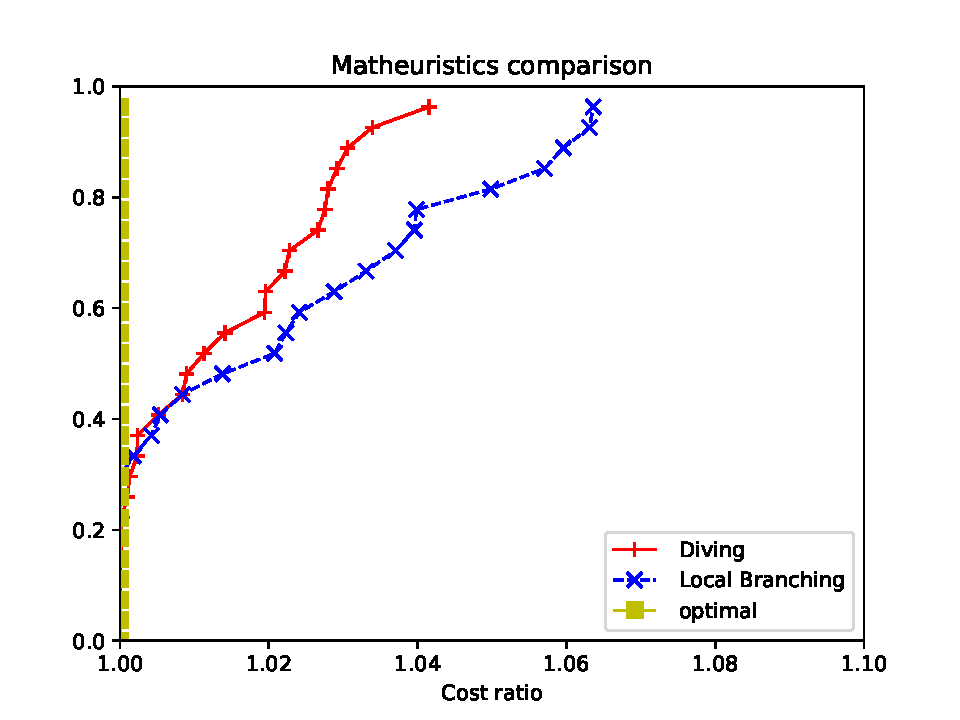
\includegraphics[width=0.7\linewidth]{Immagini/math.pdf}
    \caption{Performance profile of all Matheuristic methods.}
    \label{fig:math_comp}
\end{figure}